\chapter{Metodología y Gestión del proyecto}
\label{chap:mygp}
Este capítulo se centra en la organización del proyecto, la metodología usada y todo lo que a gestión de proyecto se refiere.
\section{Metodología}
Para el desarrollo del proyecto se ha decidido por implementar una metodología \textit{Ágile}. Este término se refiere a una metodología regida por una serie de principios que permiten ajustar la forma de trabajo a las condiciones del proyecto. Se debe priorizar a los individuos e interacciones sobre procesos y herramientas, asegurando no perder el valor humano de la comunicación no verbal en el proceso. También se debe atender antes a soluciones funcionales sobre la documentación exhaustiva. Lejos de procurar dejar de lado la documentación, es necesario tener en cuenta que el valor del desarrollo está en la funcionalidad del mismo, por lo que sacrificar tiempo de trabajo por documentar en exceso un proyecto puede acarrear resultados no deseados.
Otro pilar en el que se basa esta metodología es la respuesta al cambio sobre los planes preestablecidos, lo que asegura la versatilidad del proyecto aumentando las posibilidades de éxito.
Dada la naturaleza incremental e iterativa de la metodología \textit{Ágile} es posible dividir el ciclo de vida del proyecto en tareas para facilitar el desarrollo. Esta aproximación permite aplicar el principio de ``Divide y Vencerás'' fragmentando la estimación de las tareas y su desarrollo con el fin de reducir la dificultad en el desarrollo. En la \tablename~\ref{tab:tareas} se pueden ver todas las tareas que se llevaron a cabo junto con la estimación en horas de la misma. Destacar que dada la naturaleza del trabajo de fin de grado, se asume un único recurso humano, y por lo tanto no nos referiremos a las horas como horas por hombre o h x h.

\begin{table}
  \centering
  \rowcolors{2}{white}{udcgray!25}
  \begin{tabular}{c|c|c}
  \rowcolor{udcpink!25}
  \textbf{Nº} & \textbf{Funcionalidad}& \textbf{Estimación (H)} \\\hline
  1     &   Importar datos en formato \acrshort{dicom} en 3D Slicer.    &   2     \\
  2     &   Generar secciones para poder exportar de 3DSlicer.          &   40    \\
  3     &   Arreglar el modelo para que se viables para impresión.      &   12    \\
  4     &   Imprimir modelo.                                            &   15    \\
  5     &   Instalar librerías necesarias para el desarrollo.           &   4     \\
  6     &   Familiarizarse con la librería.                             &   12    \\
  7     &   Prototipar pruebas para tests.                              &   40    \\
  8     &   Implementar herramienta para tracking del marcador.         &   40    \\  
  9     &   Testear prototipos.                                         &   25    \\
  10    &   Generar modelo a partir el prototipo final.                 &   33    \\
  11    &   Imprimir prototipo final.                                   &   16    \\
  12    &   Instalar y compilar Exposure Render.                        &   80    \\
  13    &   Familiarizarse con el software y sistema de trabajo.        &   19    \\
  14    &   Integrar software de tracking en Exposure Render            &   24    \\
  15    &   Instalar software necesario para el \acrshort{hmd}          &   2     \\
  16    &   Familiarizarse con el uso del \acrshort{hmd}                &   24    \\
  17    &   Ejecutar pruebas de passthrough                             &   2     \\
  18    &   Integrar passthrough en Exposure Render                     &   32    \\
  
  \end{tabular}
  \caption{Tareas llevadas a cabo}
  \label{tab:tareas}
\end{table}

Para llevar a cabo las tareas se optó por un desarrollo en \textit{Sprints}. Los sprints son los períodos de tiempo en los que se llevan a cabo las tareas. Estos se acotaron en el tiempo, dándoles siempre una longitud determinada, y a su vez se acotaron en funcionalidad procurando siempre que finalicen alcanzando algún hito del proyecto. Estos bloques o \textit{Sprints} se fueron definiendo a lo largo del proyecto, adaptándose a las necesidades y riesgos del mismo.

\section{Sprints}
Tras introducir la metodología usada, vamos a detallar los Sprints que tuvieron lugar en el proyecto, las tareas, los riesgos y recursos disponibles para cada uno.
\subsection{Extracción de un modelo a partir de un \acrshort{tc}}
En este sprint, se tuvo como objetivo el desarrollo de las tareas 1, 2, 3 y 4. Dado que en el estudio previo se encontraron varios caminos disponibles para alcanzar las tareas objetivo, el sprint se consideró viable en todo momento. Este sprint se llevaron a cabo la dentro del tiempo estimado de 2 semanas. El principal riesgo fue la complejidad de la pieza, que en una impresora 3D de filamento común podría haber alargado la impresión, o incluso fallar en el proceso. Esto se minimizó utilizando la impresora Fuse 1+ 30W capaz de imprimir modelos mas complejos a pesar de tener una superficie de impresión mas reducida.

\begin{figure}
  \centering
  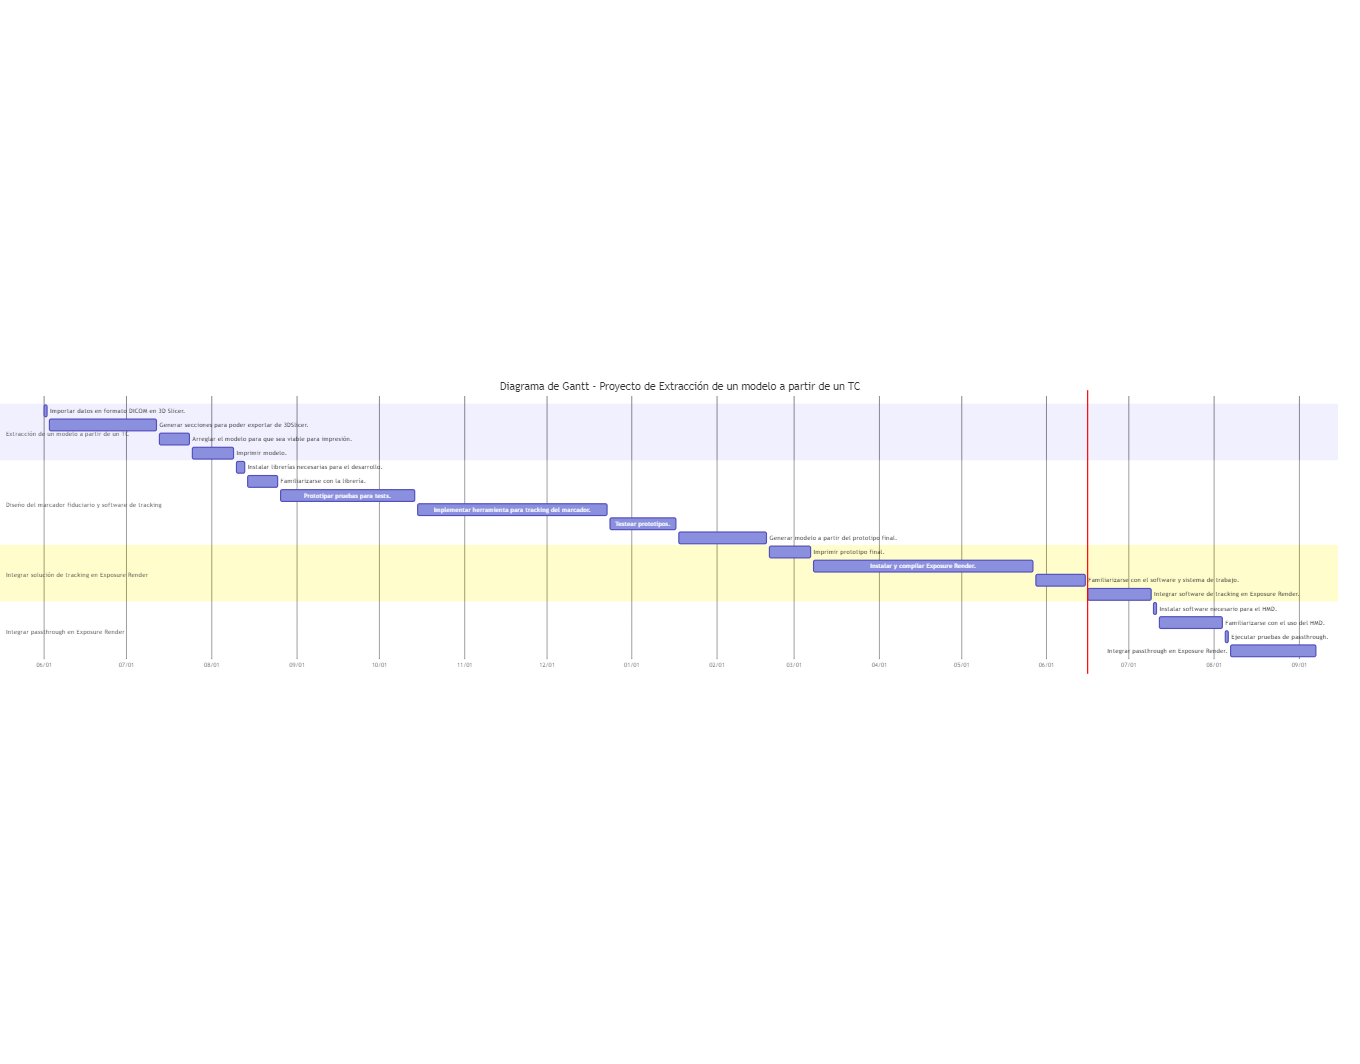
\includegraphics[angle=90, height= 1.0\textheight]{imaxes/gantt.png}
  \caption{Diagrama de la planificación del proyecto por sprints}
  \label{fig:sprint1t}
\end{figure}

\subsection{Diseño del marcador fiduciario y software de tracking}
Durante este Sprint, se llevaron a cabo las tareas de la 5 a la 10. En este caso el mayor riesgo fue el tiempo de prototipado, ya que para una única pieza a imprimir, el tiempo de impresión oscila las 15 horas. Para minimizar este riesgo se optó por realizar prototipos sobre papel como se comenta en la ejecución del proyecto. El tiempo estimado para este sprint fue de 3 semanas y media, pero debido a la dificultad de las tareas 7 y 8 se alargó a 5 semanas.

\subsection{Integrar solución de tracking en Exposure Render}
Las tareas de la 11 a la 14 se llevaron a cabo en este Sprint. La compilación e instalación de todo el software necesario para ejecutar Exposure Render fue el riesgo por excelencia de este sprint. A pesar de esto se realizo dentro del tiempo estimado para ello ya que se conocía en el momento de la planificación.

\subsection{Integrar passthrough en Exposure Render}
Se trata del ultimo sprint del proyecto, se llevaron a cabo las tareas de la 14 a la 18. En este sprint, nos encontramos con el mayor imprevisto del proyecto. El \acrshort{sdk} del \acrshort{hmd} no funcionaba correctamente, lo que imposibilitaba la reconstrucción de imágenes y causó un gran retraso en el proyecto respecto a la planificación inicial.